\documentclass[11pt]{article}
\usepackage[margin=1in]{geometry}
\usepackage{booktabs}
\usepackage{graphicx}
\usepackage{float}
\begin{document}
\section*{Supplementary Step 10 Visualization Report}
\subsection*{Overview}
\begin{tabular}{p{0.42\linewidth}p{0.50\linewidth}}
\toprule
Metric & Value\\
\midrule
Included participant-sessions & 36\\
Included questions & 30\\
Included trials & 1075\\
Primary robust SE type & Two-way cluster (participant + question)\\
Primary FE p-value & 0.209749\\
Participant-clustered p-value & 0.151850\\
Question-clustered p-value & 0.228028\\
HC3 p-value & 0.173034\\
Fixed-window benchmark p-value & 0.219180\\
No-override p-value & 0.367415\\
Back ROI benchmark p-value & 0.224774\\
Leave-one-question-out p range & 0.079410 to 0.412718\\
Leave-one-participant-out p range & 0.067180 to 0.292688\\
\bottomrule
\end{tabular}
\paragraph{Interpretation note.} In the final participant-fixed-effects robustness analysis, the abstract-versus-concrete effect in the left frontal ROI was not statistically significant (beta=3.016e-08, SE=2.351e-08, p=0.209749, 95\% CI [-1.793e-08, 7.824e-08]). Together with the non-significant sensitivity models, this suggests that the frontal condition tendency remains descriptive but does not receive robust statistical support in the current dataset.
\paragraph{Influence note.} The leave-one-question-out p-values ranged from 0.079410 to 0.412718, and the leave-one-participant-out p-values ranged from 0.067180 to 0.292688. Neither influence analysis produced any p-value below 0.05.
\subsection*{Core Step 10 Figures}
\begin{figure}[H]
\centering
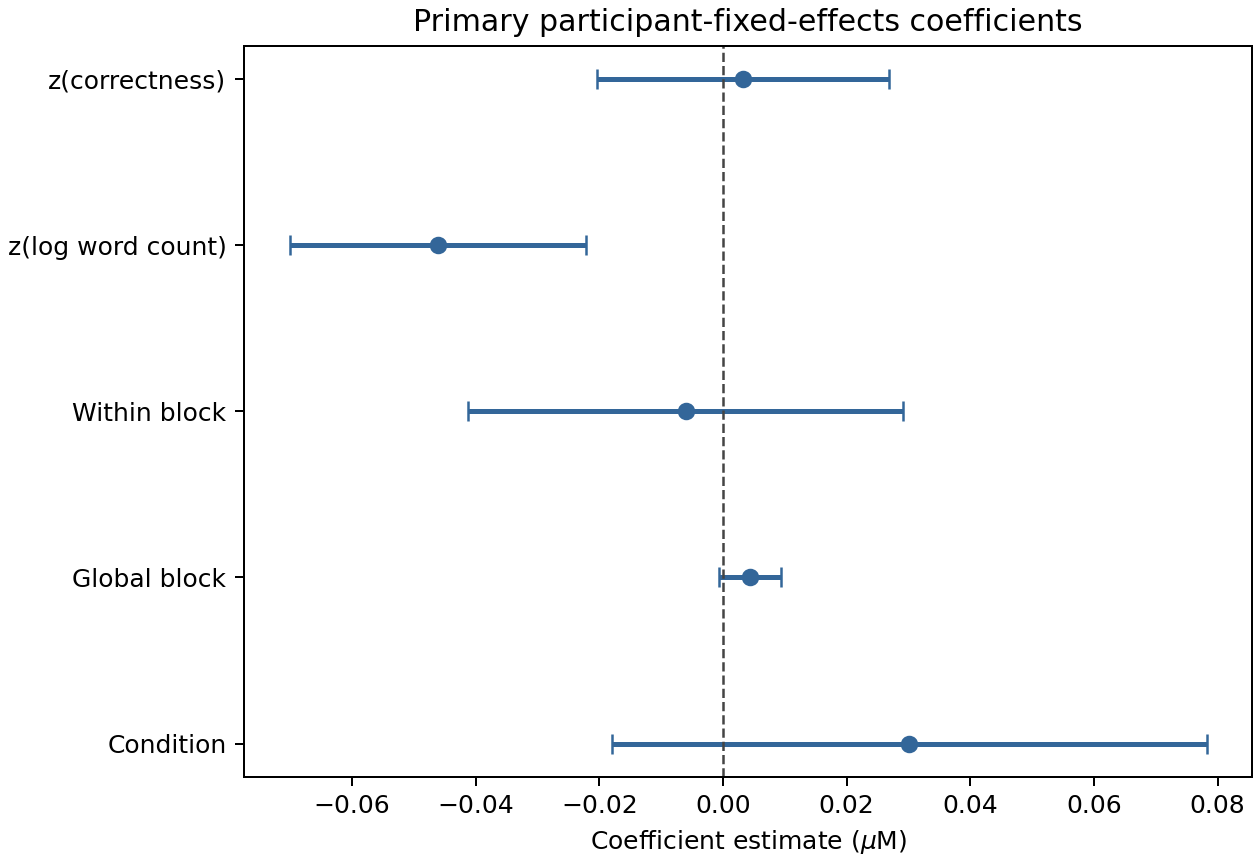
\includegraphics[width=0.48\linewidth]{../../figures/step10/primary_condition_coefficient_plot.png}
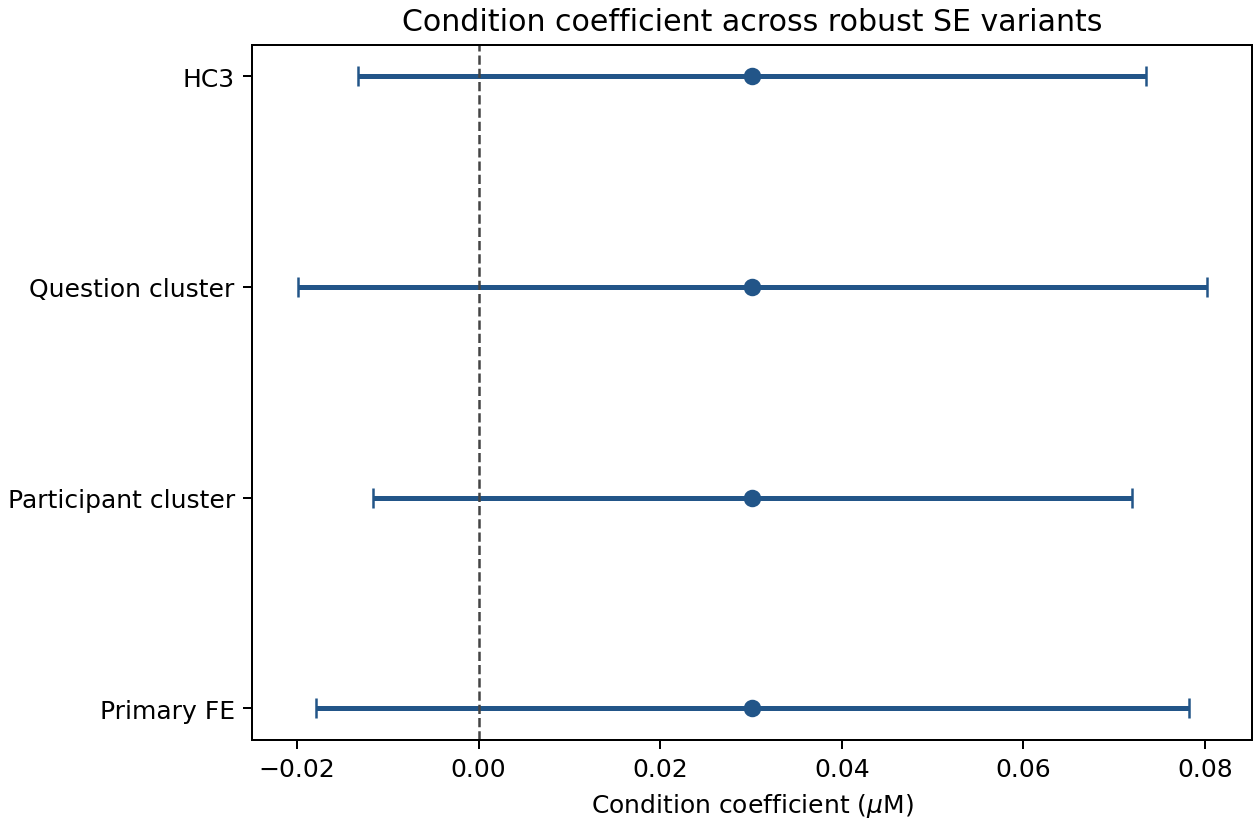
\includegraphics[width=0.48\linewidth]{../../figures/step10/robust_se_comparison.png}
\caption{Primary participant-fixed-effects coefficient summary and the robust-standard-error comparison.}
\end{figure}
\begin{figure}[H]
\centering
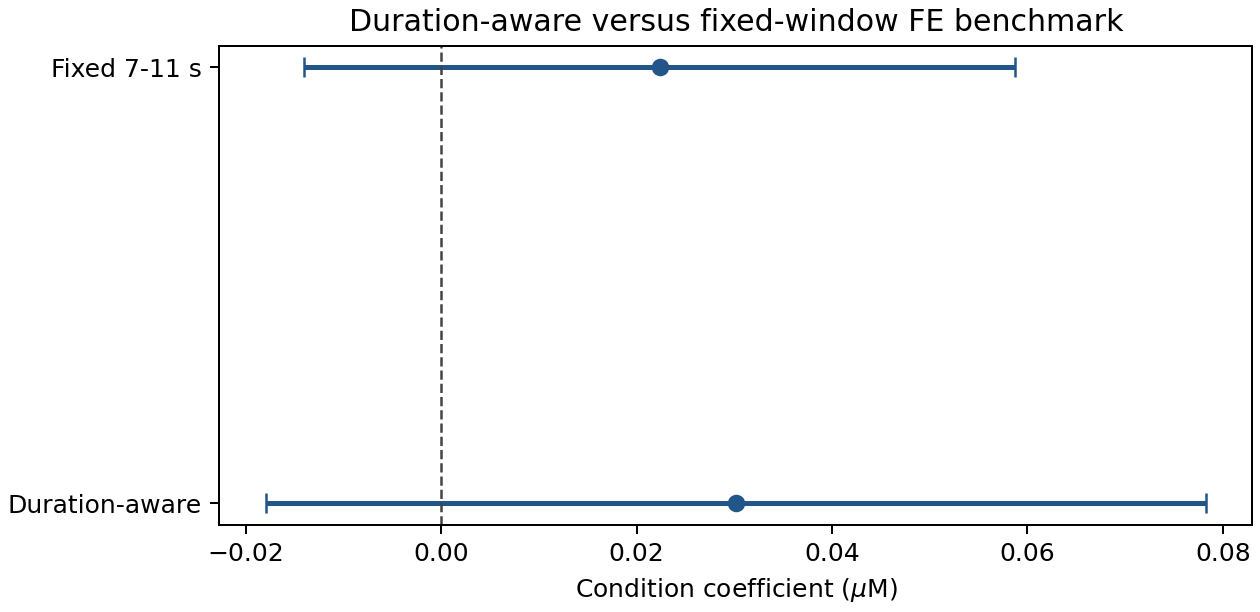
\includegraphics[width=0.48\linewidth]{../../figures/step10/fixed_vs_variable_fe_benchmark.png}
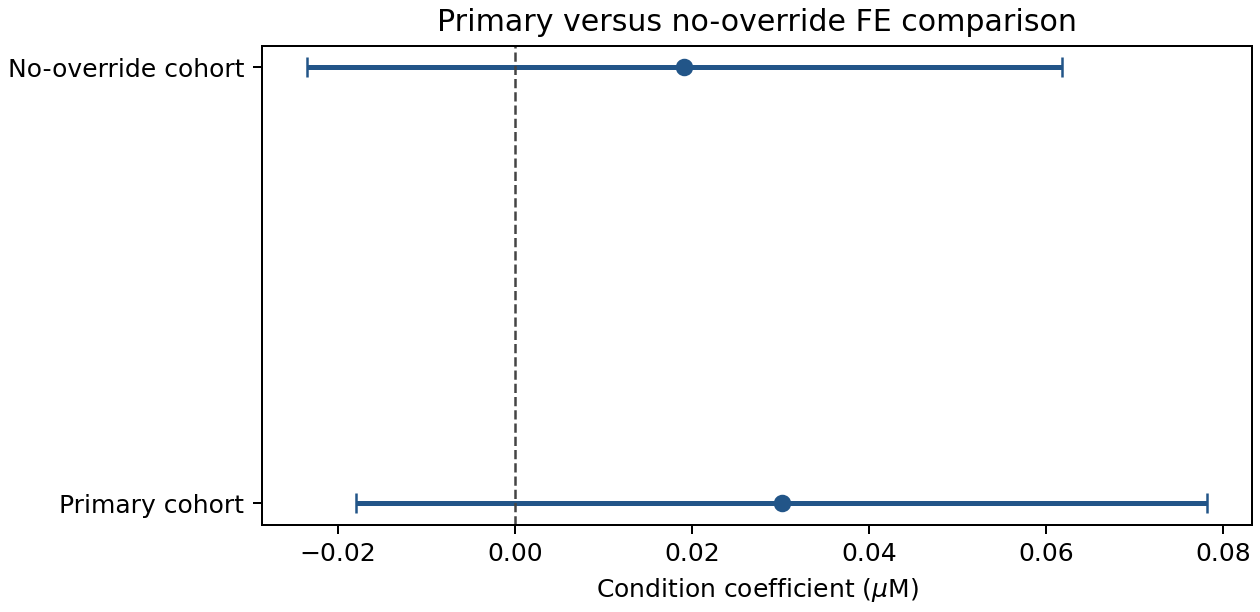
\includegraphics[width=0.48\linewidth]{../../figures/step10/no_override_comparison.png}
\caption{Duration-aware versus fixed-window benchmark and the no-override sensitivity comparison.}
\end{figure}
\begin{figure}[H]
\centering
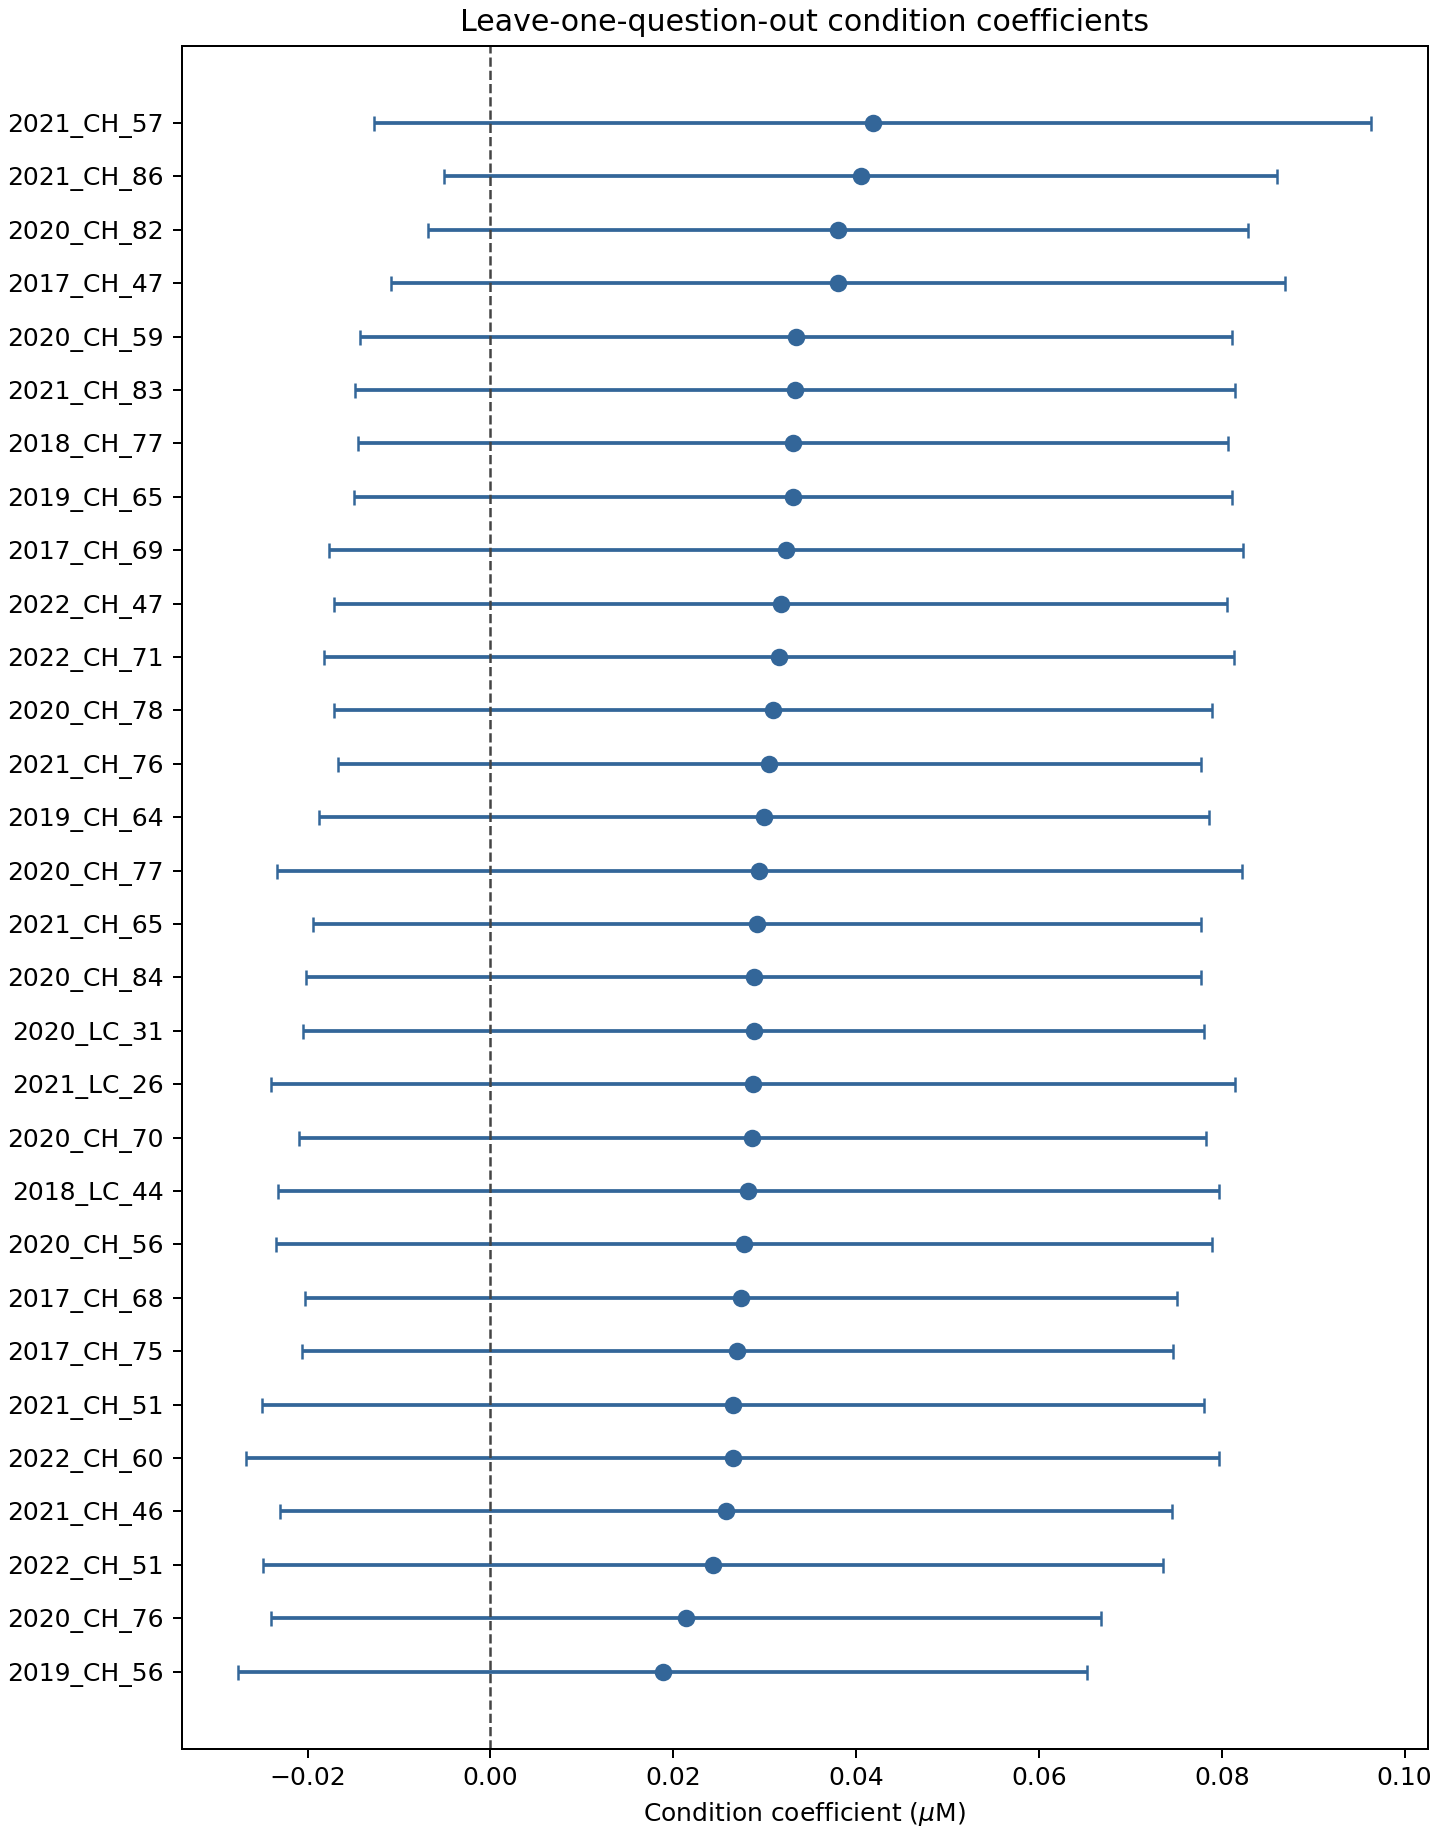
\includegraphics[width=0.48\linewidth]{../../figures/step10/leave_one_question_out_plot.png}
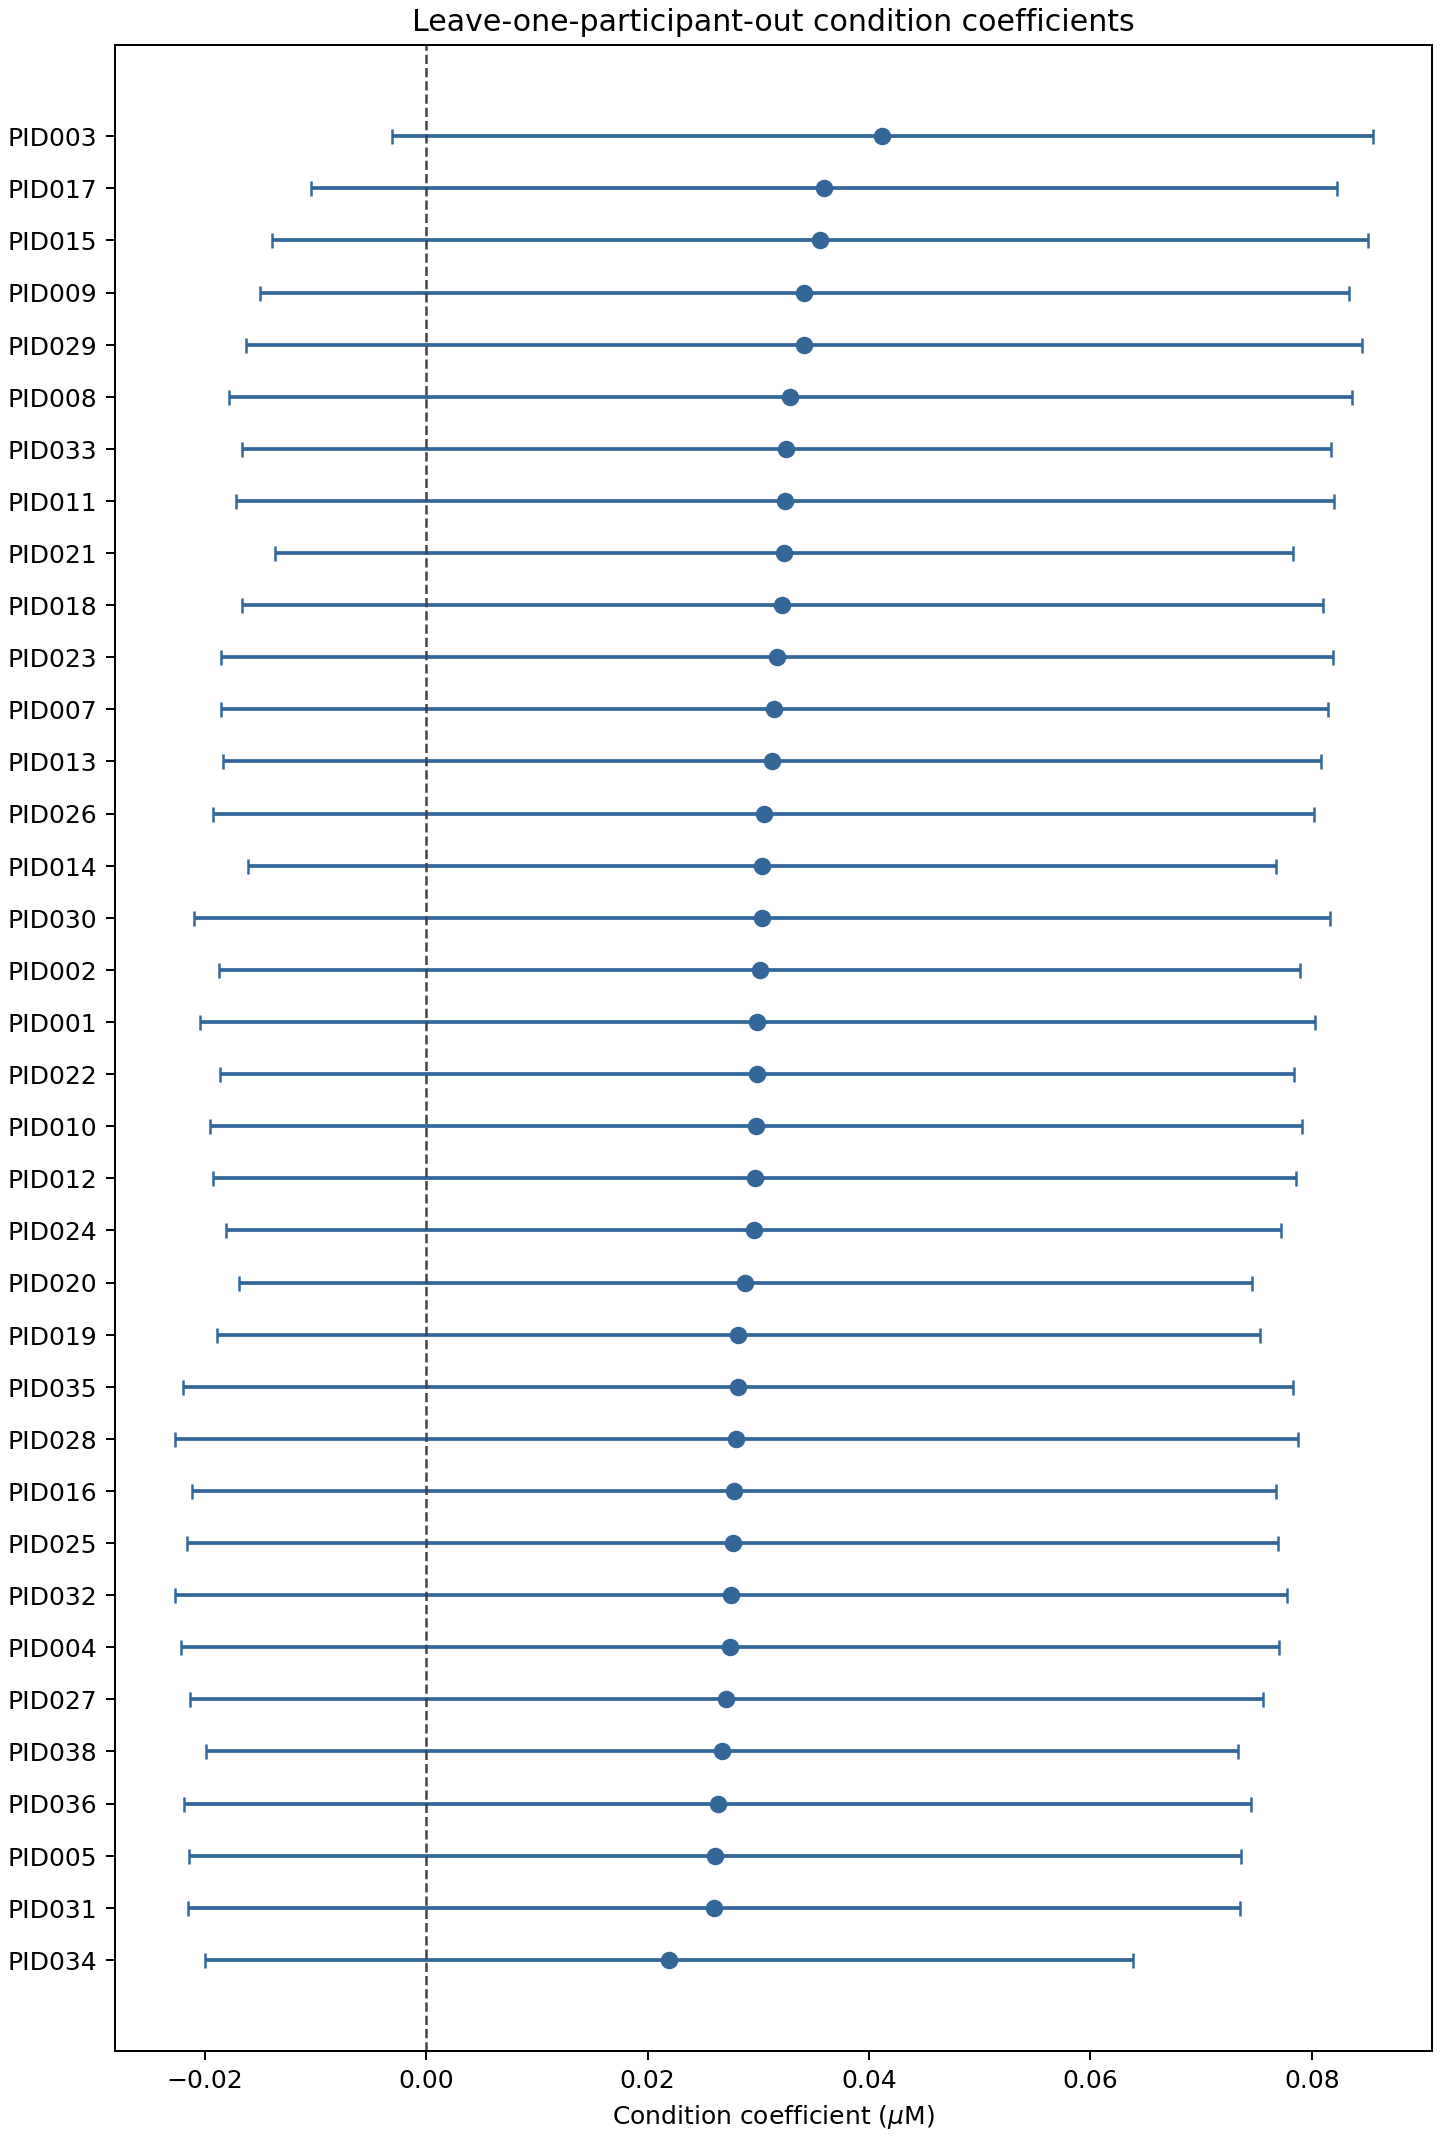
\includegraphics[width=0.48\linewidth]{../../figures/step10/leave_one_participant_out_plot.png}
\caption{Condition coefficients from the leave-one-question-out and leave-one-participant-out influence analyses.}
\end{figure}
\subsection*{Additional Influence Diagnostics}
\begin{figure}[H]
\centering
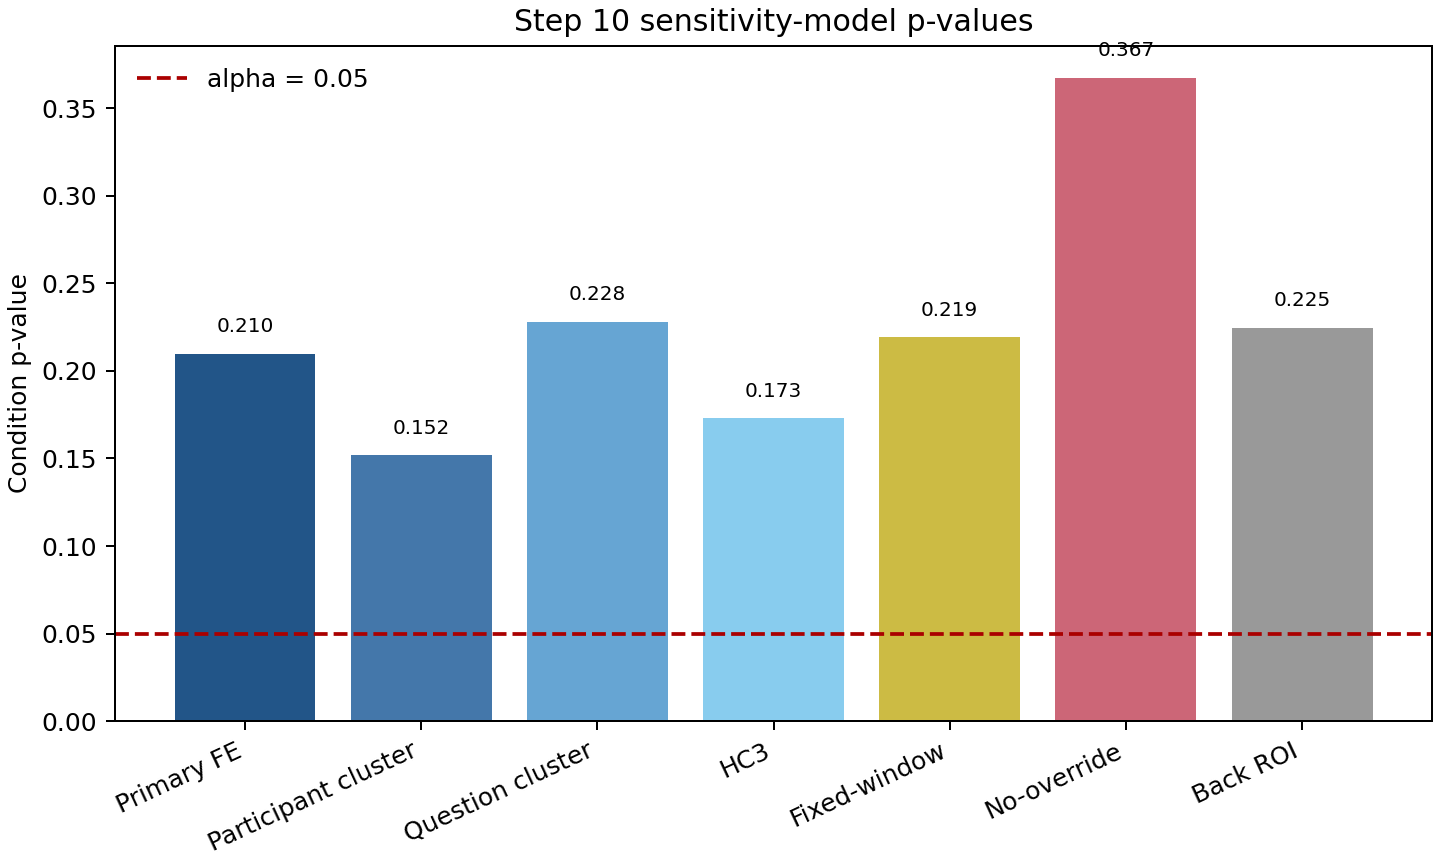
\includegraphics[width=0.90\linewidth]{../../figures/step10_visualization/sensitivity_pvalue_summary.png}
\caption{Condition p-values across the primary and sensitivity Step~10 models.}
\end{figure}
\begin{figure}[H]
\centering
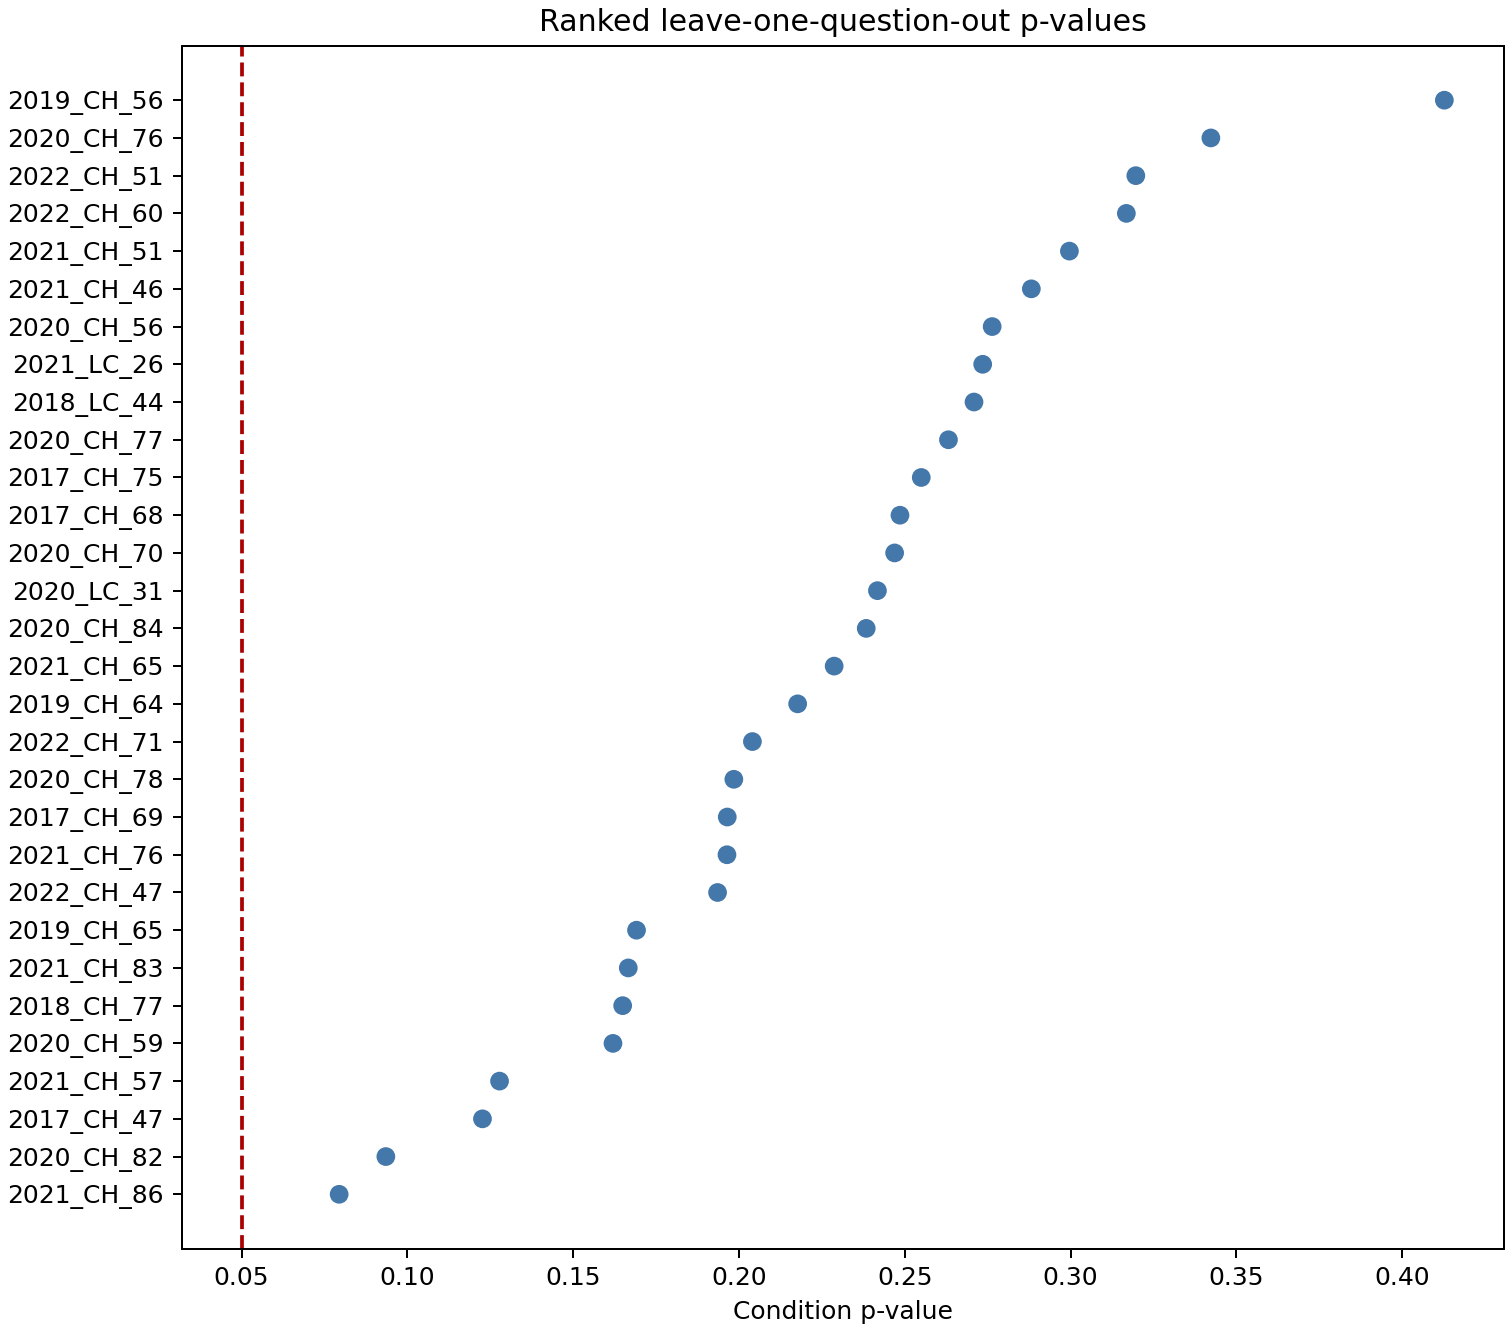
\includegraphics[width=0.48\linewidth]{../../figures/step10_visualization/leave_one_question_out_pvalues.png}
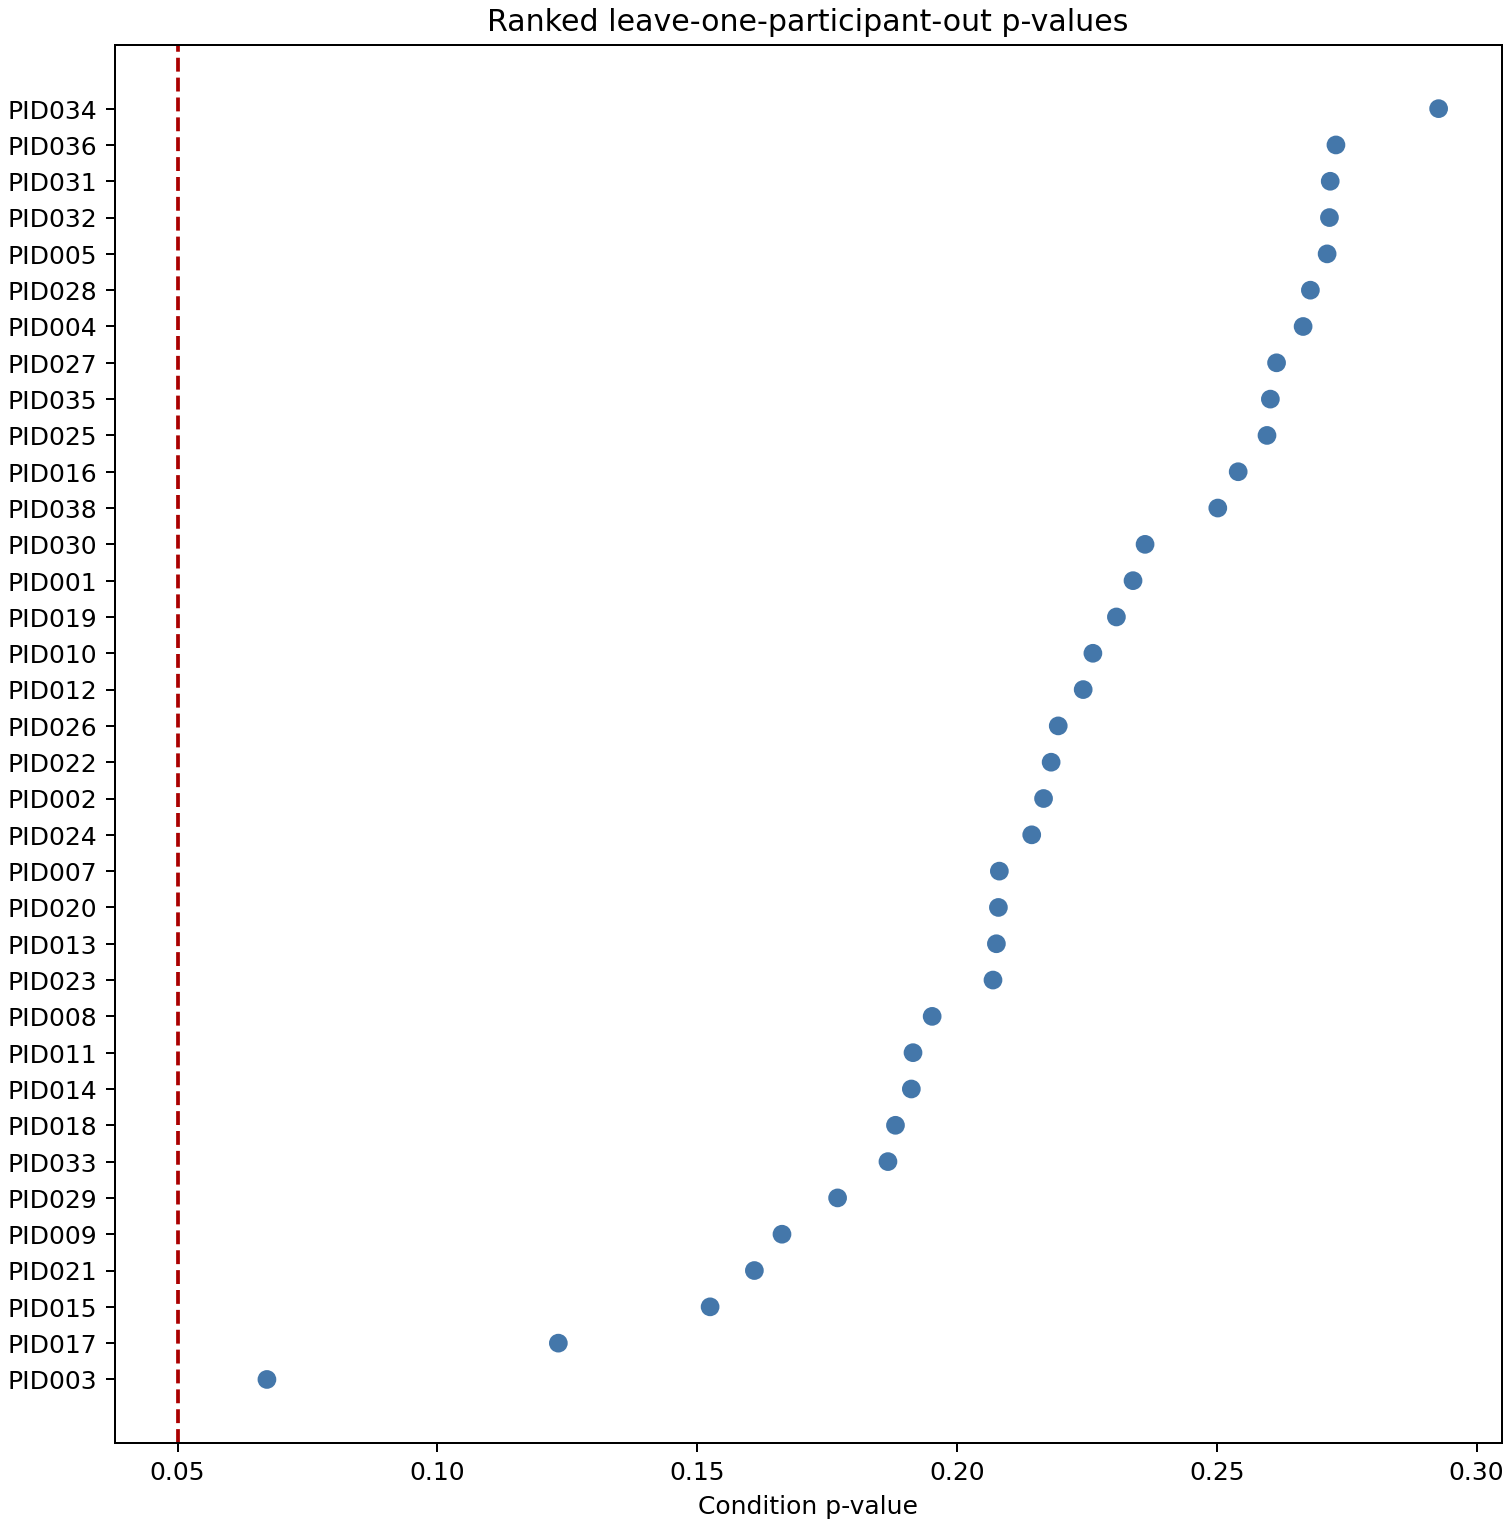
\includegraphics[width=0.48\linewidth]{../../figures/step10_visualization/leave_one_participant_out_pvalues.png}
\caption{Ranked p-values from the leave-one-question-out and leave-one-participant-out analyses. The red line marks alpha=0.05.}
\end{figure}
\end{document}
